\documentclass{book}
\usepackage{wrapfig}
\usepackage{graphicx}
\usepackage{tikz-timing}
\usepackage{listings}
%\usepackage{biblatex}
%\addbibresource{mainframe.bib}
\begin{document}
\frontmatter
\title{Documentation for z80 Mainframe}
\author{Colton Beck}
\maketitle
\section*{Legal Information}
\subsection*{Disclaimer of Warranty}

  THERE IS NO WARRANTY FOR THE PROGRAM, TO THE EXTENT PERMITTED BY
APPLICABLE LAW.  EXCEPT WHEN OTHERWISE STATED IN WRITING THE COPYRIGHT
HOLDERS AND/OR OTHER PARTIES PROVIDE THE PROGRAM "AS IS" WITHOUT WARRANTY
OF ANY KIND, EITHER EXPRESSED OR IMPLIED, INCLUDING, BUT NOT LIMITED TO,
THE IMPLIED WARRANTIES OF MERCHANTABILITY AND FITNESS FOR A PARTICULAR
PURPOSE.  THE ENTIRE RISK AS TO THE QUALITY AND PERFORMANCE OF THE PROGRAM
IS WITH YOU.  SHOULD THE PROGRAM PROVE DEFECTIVE, YOU ASSUME THE COST OF
ALL NECESSARY SERVICING, REPAIR OR CORRECTION.

\subsection*{Limitation of Liability}

  IN NO EVENT UNLESS REQUIRED BY APPLICABLE LAW OR AGREED TO IN WRITING
WILL ANY COPYRIGHT HOLDER, OR ANY OTHER PARTY WHO MODIFIES AND/OR CONVEYS
THE PROGRAM AS PERMITTED ABOVE, BE LIABLE TO YOU FOR DAMAGES, INCLUDING ANY
GENERAL, SPECIAL, INCIDENTAL OR CONSEQUENTIAL DAMAGES ARISING OUT OF THE
USE OR INABILITY TO USE THE PROGRAM (INCLUDING BUT NOT LIMITED TO LOSS OF
DATA OR DATA BEING RENDERED INACCURATE OR LOSSES SUSTAINED BY YOU OR THIRD
PARTIES OR A FAILURE OF THE PROGRAM TO OPERATE WITH ANY OTHER PROGRAMS),
EVEN IF SUCH HOLDER OR OTHER PARTY HAS BEEN ADVISED OF THE POSSIBILITY OF
SUCH DAMAGES.
\chapter*{Dedication}
Dedicated to caffeine for giving me the energy to write this and sleep deprivation for making me think this was a good idea.
\tableofcontents
\listoffigures
\listoftables
\mainmatter
\chapter{Main Board}
The system is designed to use one higher wattage power supply to provide the low voltage for the peripherals and main board. For the system as shown here, the supply should be rated at least seven amperes at five volts and fifteen amperes at twelve volts for a combined two hundred fifteen watts of total power. If additional peripherals are expected to be added, then the power suppy should be of a higher wattage so that the whole system can be powered from a unified supply to avoid the risk of ground loops that could induce exxecive noise.

For the rear panel power connections, any connectors may be used but it is advised to use incompatable connectors for the low voltage and high voltage connections to avoid accidental interconnection. For this reason, the parts list specifies NEMA L5-15 plugs and recepticals for the high voltage and NEMA L5-20 plugs and recepticals for the low voltage(See Table~\ref{tab:partlist} on pg~\pageref{tab:partlist})

For the data connections, it is recomended to use 

\begin{wrapfigure}{R}{0.5\textwidth}
  \begin{center}
    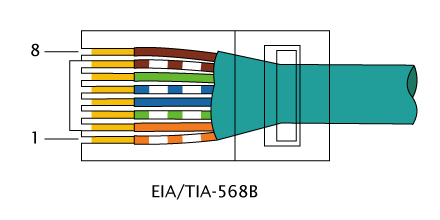
\includegraphics[width=0.48\textwidth]{RJ-45_TIA-568B_Left.png}
  \end{center}
  \caption{Example wiring using EIA-568B\cite{img:eia568}\label{fig:eia568}}
\end{wrapfigure}

\begin{table}
\centering
\begin{tabular}{| l | l | l |}
Pin Number & Function & Wire Color\\
1 & Tx- & White/Orange\\
2 & Tx+ & Orange\\
3 & TxClk- & White/Green\\
4 & RxClk+ & Blue\\
5 & RxClk- & White/Blue\\
6 & TxClk+ & Green\\
7 & Rx- & White/Brown\\
8 & Rx+ & Brown\\
\end{tabular}
\caption{Interface Pin Functions\label{tab:intpin}}
\end{table}
The inter-peripheral communication is done via a differential serial link over 4 pair u/utp cabling in a full duplex configuration. This link is cloked at 40MHz limited by the maximum bandwidth of the shift register and differential driver. This link is designed to be wired as illustrated in figure \ref{fig:eia568} and in table \ref{tab:intpin}. Either of EIA-568A or B or some other wiring scheme may be used as long as the pinout is preserved. It is reccomended to keep the differential signal pairs on twisted pairs to minimize crosstalk and interference since the link has a high data rate and interference could be detrimental to the operation of the system.

Using a parallel connection would allow for a higher throughput however this comes at a highercost due to the cost of connectors and cabling. Hardware limitations in the serial to parallel converter limit the maximum clock speed of the z80 since all 31 lines needed for peripheral communication need to be sent every clock cycle due to the z80 having an inconsistent number of clock cycles per instruction. This limits the z80 to a clock speed of 1.25MHz since there are 31 bits plus a start/stop bit being sent at 40Mbit/s. If the shift registers and differential tranceivers specified in Appendix A cannot be acquired, lower speed components may be used however, the colck speed of the z80 must be lowered accordingly.

The z80 mainframe was designed to be modular and expandable. It acomplishes this by having a simple interface that brings out the lines from the main bus necessary for IO control and direct memory access. The system is limited to 232 connected peripherals because of the limitations of the z80's IO addressing technique. The z80 only uses the lower 8 bits of the address bus for IO addressing while the contents of the accumulator are placed on the upper 8 bits in teh case of  the IN A,(n) instruction\cite[p.~295]{zlg:z80}

The peripherals  are designed to look for a specific address after which the device pulls the BUSREQ line low and reads from 0x0800 to 0x084F or writes to 0x850 to 0x089F. The peripherals listed here are designed to be configurable as to what address they respond to and the OS is configurable for where it is trying to address these devices at. Both are configured in hardware rather than in software to simplify configuration co the OS can determine settings without the ROM needing to be modified to be instalation dependant.

\chapter{Dot Matrix Printer}
The main output for the z80 mainframe is the printer. This particular setup is designed to use an Epson LX-810 printer interfacing over a parallel port as shown in figure~(null pointer).
\begin{figure}[h]
\centering
\begin{tikztimingtable}
$\mathrm{DATA\:0-7}$         &   UU7D{\textnormal{MEM 0x0800}}7D{\textnormal{MEM 0x0801}}XX7D{\textnormal{MEM 0x0850}}7D{\textnormal{0x0D}}UU\\
$\overline{\mathrm{STROBE}}$ &   HHHLHHHHHHLHHHHHXXHLHHHHHHLHHHHHHH\\
$\overline{\mathrm{BUSY}}$   &   HHHHHHHHLHHHHHHLXXHHHHHHLHHHHHHLHH\\
\end{tikztimingtable}
\caption{Driver Board to Printer Timing}
\label{fig:lptiming}
\end{figure}
\begin{figure}[h]
\centering
\begin{tikztimingtable}
$\mathrm{ADDR\:0-15}$          &   U8D{\textnormal{0x00FB}}UU6D{\textnormal{0x0800}}XXX6D{\textnormal{0x0850}}UUUU\\
$\mathrm{DATA\:0-7}$           &   UU7D{\textnormal{Option Byte}}UUXX4D{\textnormal{Data}}XXXXX4D{\textnormal{In}}UUUU\\
$\overline{\mathrm{WAIT}}$    &   UUUULLLLHHHHHHHHHHHHHHHHHHHHHU\\
$\overline{\mathrm{MREQ}}$    &   UHHHHHHHHHHHLLLLLHXXHLLLLLHHHU\\
$\overline{\mathrm{IORQ}}$    &   UHHLLLLHHHHHHHHHHHHHHHHHHHHHHU\\
$\overline{\mathrm{RD}}$      &   UHHHHHHHHHHHLLLLLHXXHLLLLLHHHU\\
$\overline{\mathrm{WR}}$      &   UHHLLLLHHHHHHHHHHHHHHHHHHHHHHU\\ 
$\overline{\mathrm{BUSREQ}}$  &   UHHHHHLLLLLLLLLLLLLLLLLLLLLHHH\\
$\overline{\mathrm{BUSACK}}$  &   UHHHHHHLLLLLLLLLLLLLLLLLLLLLHH\\
\extracode
\begin{pgfonlayer}{background}
\vertlines[help lines]{1,2,3,4,5,6,7,8,9,10,11,12,13,14,15,16,17,18,19,20,21,22,23,24,25,26,27,28,29,30}
\end{pgfonlayer}
\end{tikztimingtable}
\caption{Main Bus to Printer Driver Timing}
\label{fig:lpdrivertiming}
\end{figure}
\chapter{Card Punch \& Reader}
\chapter{Paper Tape Punch \& Reader}
\appendix
\chapter{Part List}
\begin{tabular}{| l | l | l | r | r | r |}
\hline
\label{tab:partlist}
Source & Part Number & Description & Quantity & Price/each & Line Total \\ \hline
McMaster & 7162K29 & L5-15P Cable Mount & 1 & \$9.15 & \$9.15\\ \hline
McMaster & 7162K32 & L5-15R Cable Mount & 2 & \$16.29 & \$32.58\\ \hline
McMaster & 7162K8 & L5-15P Panel Mount & 2 & \$12.06 & \$24.12\\ \hline
McMaster & 7162K77 & L5-15R Panel Mount & 1 & \$16.00 & \$9.15\\ \hline
McMaster & 7162K36 & L5-20P Cable Mount & 5 & \$11.59 & \$57.95\\ \hline
McMaster & 7162K38 & L5-20R Cable Mount & 5 & \$18.00 & \$90.00\\ \hline
McMaster & 7162K9 & L5-20P Panel Mount & 3 & \$14.65 & \$43.95\\ \hline
McMaster & 7162K94 & L5-20R Panel Mount & 5 & \$20.59 & \$102.95\\ \hline
McMaster & 7422K22  & 16/3 SJOOW Cable & 70 & \$0.72/ft & \$50.40\\ \hline
Mouser & ATMEGA328 & 8-bit Microcontroler & 5 & \$1.96 & \$9.80\\ \hline
Mouser & Z84C0010PEG & CMOS Z80 CPU & 1 & \$5.36 & \$5.36\\ \hline
Mouser & AT28C64B-15PU & 8Kx8 EEPROM & 1 & \$3.13 & \$3.13\\ \hline
Mouser & 71256SA12TPG & 32Kx8 SRAM & 2 & \$3.13 & \$6.26\\ \hline
MFN & PN & Desc & 0 & \$0.00 & \$0.00\\ \hline
\end{tabular}
\chapter{Code Listings}
\lstset{numbers=left, numberstyle=\tiny, stepnumber=1, numbersep=5pt}
\section{ROM Listing}
\cleardoublepage
\section{Line Printer Driver Listing}
\lstinputlisting[language=C++,firstline=3]{../Code/PrinterDriver/PrinterDriver.ino}
\cleardoublepage
\section{Card Punch Driver Listing}
\cleardoublepage
\section{Card Reader Driver Listing}
\cleardoublepage
\section{Paper Tape Punch Driver Listing}
\cleardoublepage
\section{Paper Tape Reader Driver Listing}
\chapter{Circuit Diagrams}
\section{Main Board}
\cleardoublepage
\section{Line Printer Driver Board}
\cleardoublepage
\section{Card Punch \& Reader Driver Board}
\cleardoublepage
\section{Paper Tape Punch \& Reader Driver Board}
\chapter{PCB Masks}
\section{Main Board}
\cleardoublepage
\section{Line Printer Driver Board}
\cleardoublepage
\section{Card Punch \& Reader Driver Board}
\cleardoublepage
\section{Paper Tape Punch \& Reader Driver Board}
\chapter{Part Drawings}
\backmatter
\bibliographystyle{plain}
\addcontentsline{toc}{chapter}{Bibliography}
\bibliography{mainframe}
\cleardoublepage
\section*{Fonts}
This was typeset in Computer Modern using pdf\LaTeX{} and bib\TeX{}.
The timing diagrams were made with the tikz-timing package.
The code listings were made with the listings package
\end{document}